\documentclass[12pt]{article}
\usepackage[utf8]{inputenc}
\usepackage[T1]{fontenc}
\usepackage{amsmath,amsfonts,amssymb}
\usepackage{graphicx}
\usepackage{a4wide}

\usepackage{natbib}
\usepackage{hyperref} 
\usepackage{float}

\usepackage{algorithm}
\usepackage{algpseudocode}
\usepackage{subcaption}


\hypersetup{
    colorlinks=true,
    linkcolor=blue,
    citecolor=blue,
    urlcolor=blue
}

\bibliographystyle{apalike}



\title{Leveraging Adaptive Loss Scaling for Noisy Label Filtering}
\author{Kirill Pupkov, Igor Ignashin, Aleksandr Beznosikov}
\date{2025}
\begin{document}
\maketitle

\begin{abstract}

    In machine learning, numerous challenges can degrade model performance, including noisy features and incorrect labeling in the training data. In this paper, we investigate the use of Adaptive Loss Scaling to address these issues. Our method is more effective at separating clean and noisy labels than standard empirical risk minimization. We demonstrate the effectiveness of our approach on the CIFAR10 dataset with a fraction of noisy labels.

\end{abstract}

\section{Introduction}

Machine learning models are often applied under the assumption that training data are correctly labeled and accurately represent the true data distribution. However, in practice, training sets often contain noisy labels, negatively affecting model performance. Recent work has also shown that sufficiently large convolutional networks can easily fit a random labeling of training data \citep{zhang2017understanding}. Various approaches have been proposed in the literature to address the problem of noisy labels in training data.

One particular family of approaches focuses on reweighting training examples. Some methods utilize meta-learning to learn these weights \citep{ren2018learning}, while others use specialized networks to determine them \citep{jiang2018mentornet}. However, such methods usually rely on the availability of a smaller clean training set, which is not always present. Recent work \citep{also} discusses how the task of assigning weights can be formulated as a min-max optimization problem and proposes a method for solving it using the ALSO optimizer. Notably, it does not require any clean set and can be used as a drop-in replacement for Adam \citep{kingma2014adam} optimizer.

Other approaches focus on modifying the loss function to be more robust to label noise. \citet{bootstrap} proposed a "bootstrapping" approach that includes model predictions into the loss function to prevent overfitting. \citet{UnsupervisedLabelNoise} later added dynamic coefficients to this approach using unsupervised loss modelling. \citet{selc} further improved this approach by using ensembled model predictions from previous epochs. 

In this paper, we propose a method to leverage the weights learned by a model trained with a slightly modified version of the ALSO optimizer to accurately identify mislabeled training examples.

The main contributions of our paper include:
\begin{itemize}
    \item \textbf{A new method for label filtering.} We propose a novel approach for detecting mislabeled examples using the ALSO optimizer.
    \item \textbf{Empirical evaluation.} We extensively evaluate our approach and compare it against baseline.
\end{itemize}

\section{Preliminaries}

\subsection{Supervised Classification}
We address a $C$-class supervised classification task.
Let $\mathcal{X} \subset \mathbb{R}^d$ be the input feature space and $\mathcal{Y} \subset \{0,1\}^C$ the one-hot encoded label space. We are given a training set $D = \{(x_i, y_i)\}_{i=1}^N$. Our goal is to find $\theta \in \Theta \subset \mathbb{R}^k$ such that $q_\theta: \mathcal{X} \to \mathbb{R}^C$ minimizes an empirical risk, solving the following optimization problem:

\begin{equation}
    \min_{\theta \in \Theta} \left\{
        \frac{1}{N}\sum_{i=1}^{N} f_i(\theta) + \frac{\tau}{2}\|\theta\|_2^2
    \right\},
    \label{eq:empirical}
\end{equation}

Where $f_i(\theta) = \ell(y_i, q_\theta(x_i))$ for a chosen loss function $\ell$, typically cross-entropy. \(\tau > 0\) is a regularization parameter, and \(\frac{\tau}{2}\|\theta\|_2^2\) is the regularization term to prevent overfitting.

\subsection{Noisy Labels}
The challenge addressed in this paper is learning from a noisy training set $\tilde{D} = \{(x_i, \tilde{y}_i)\}_{i=1}^N$, where labels $\tilde{y}_i$ are potentially corrupted versions of the true labels $y_i$ with some probability $\eta$.

Minimizing empirical risk (\ref{eq:empirical}) via SGD can lead to overfitting on the mislabeled examples, degrading model performance. Following \citet{selc}, we observe the existence of a so-called "turning point", before which the model learns predominantly from clean examples, but after which it starts memorizing noisy labels (Figure~\ref{fig:memorization}).

\begin{figure}[htbp]
  \centering
  \begin{subfigure}[b]{0.45\textwidth}
    \centering
    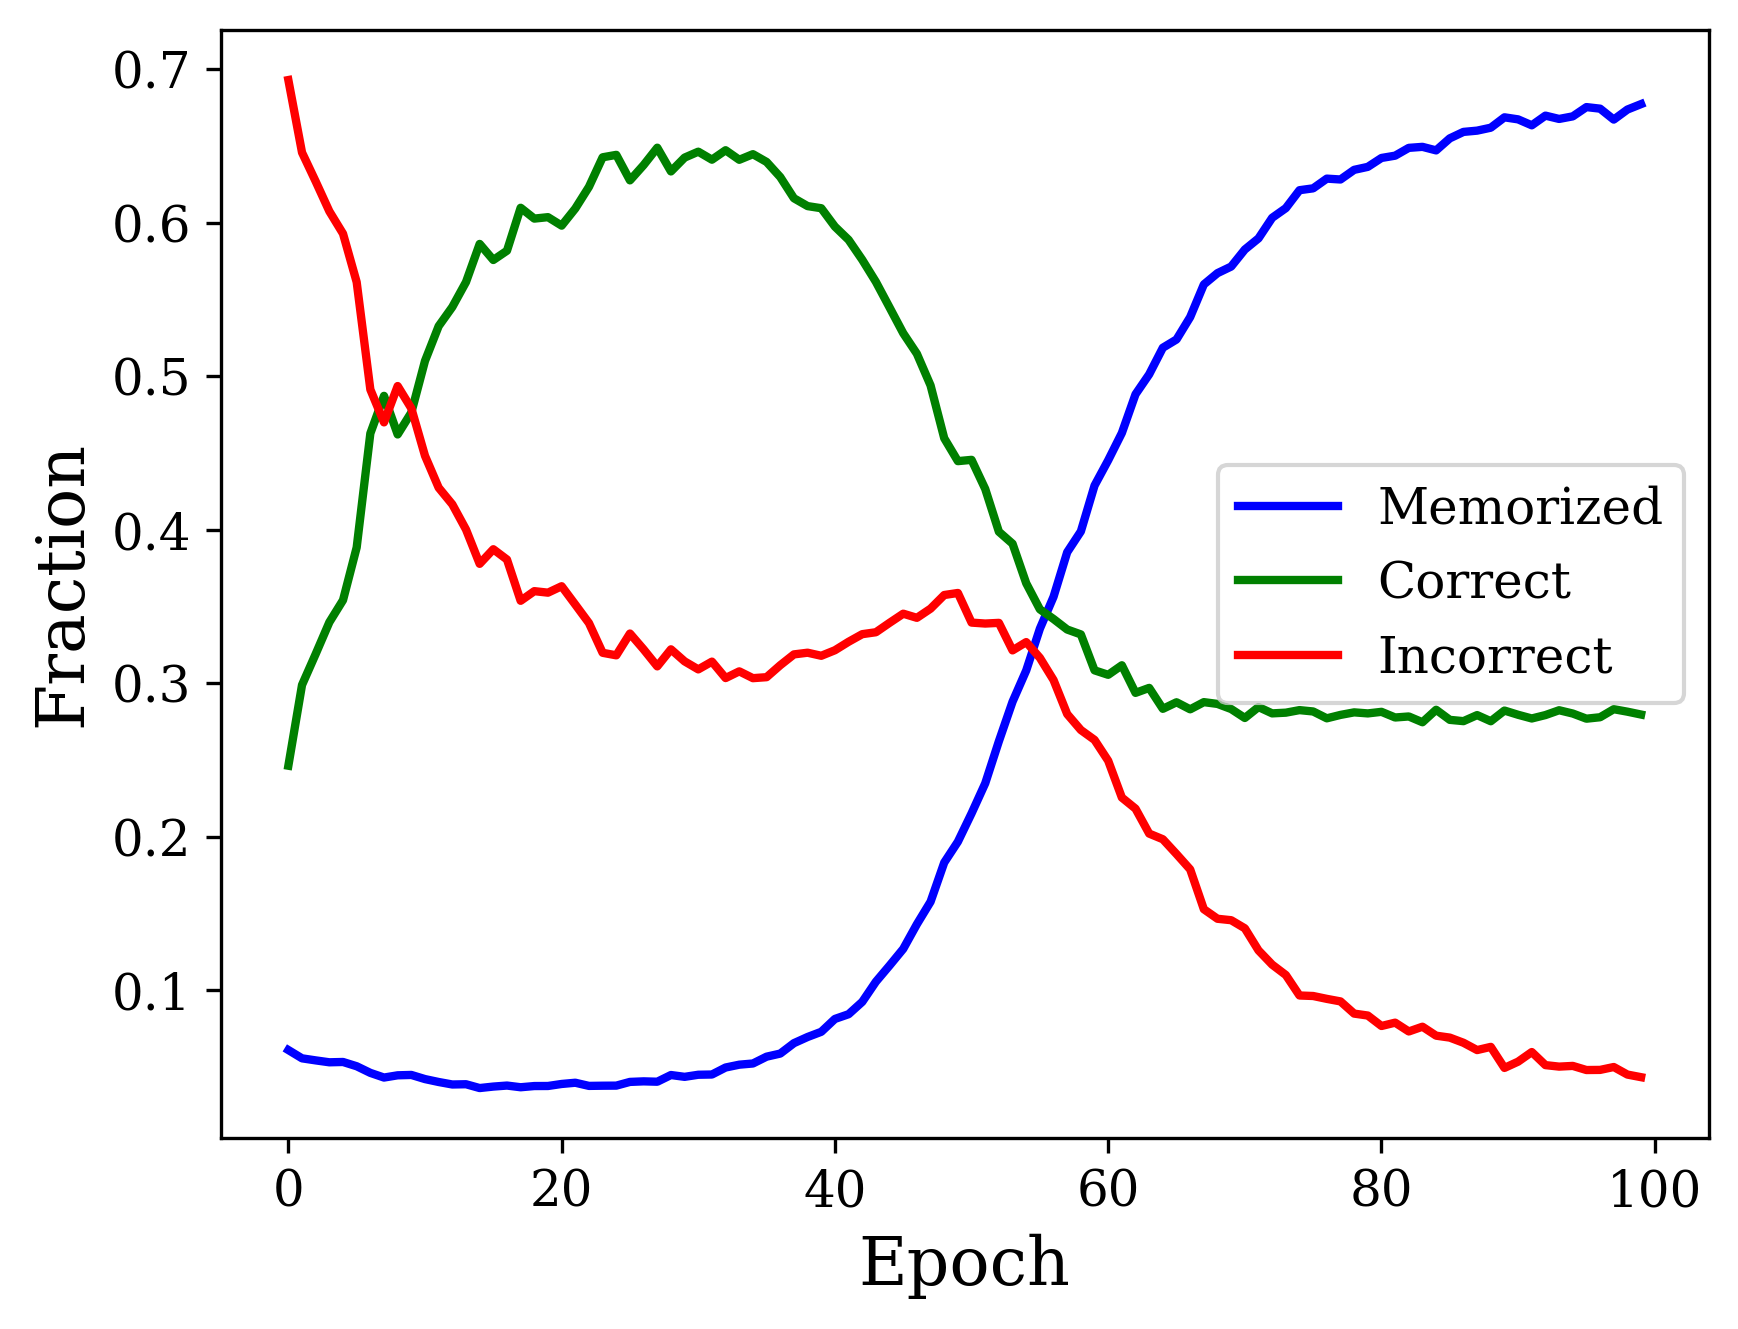
\includegraphics[width=\textwidth]{figures/memorized_correct_incorrect_08.png}
    \caption{symmetric noise, $\eta=0.8$}
    \label{fig:sub1}
  \end{subfigure}
  \hfill
  \begin{subfigure}[b]{0.45\textwidth}
    \centering
    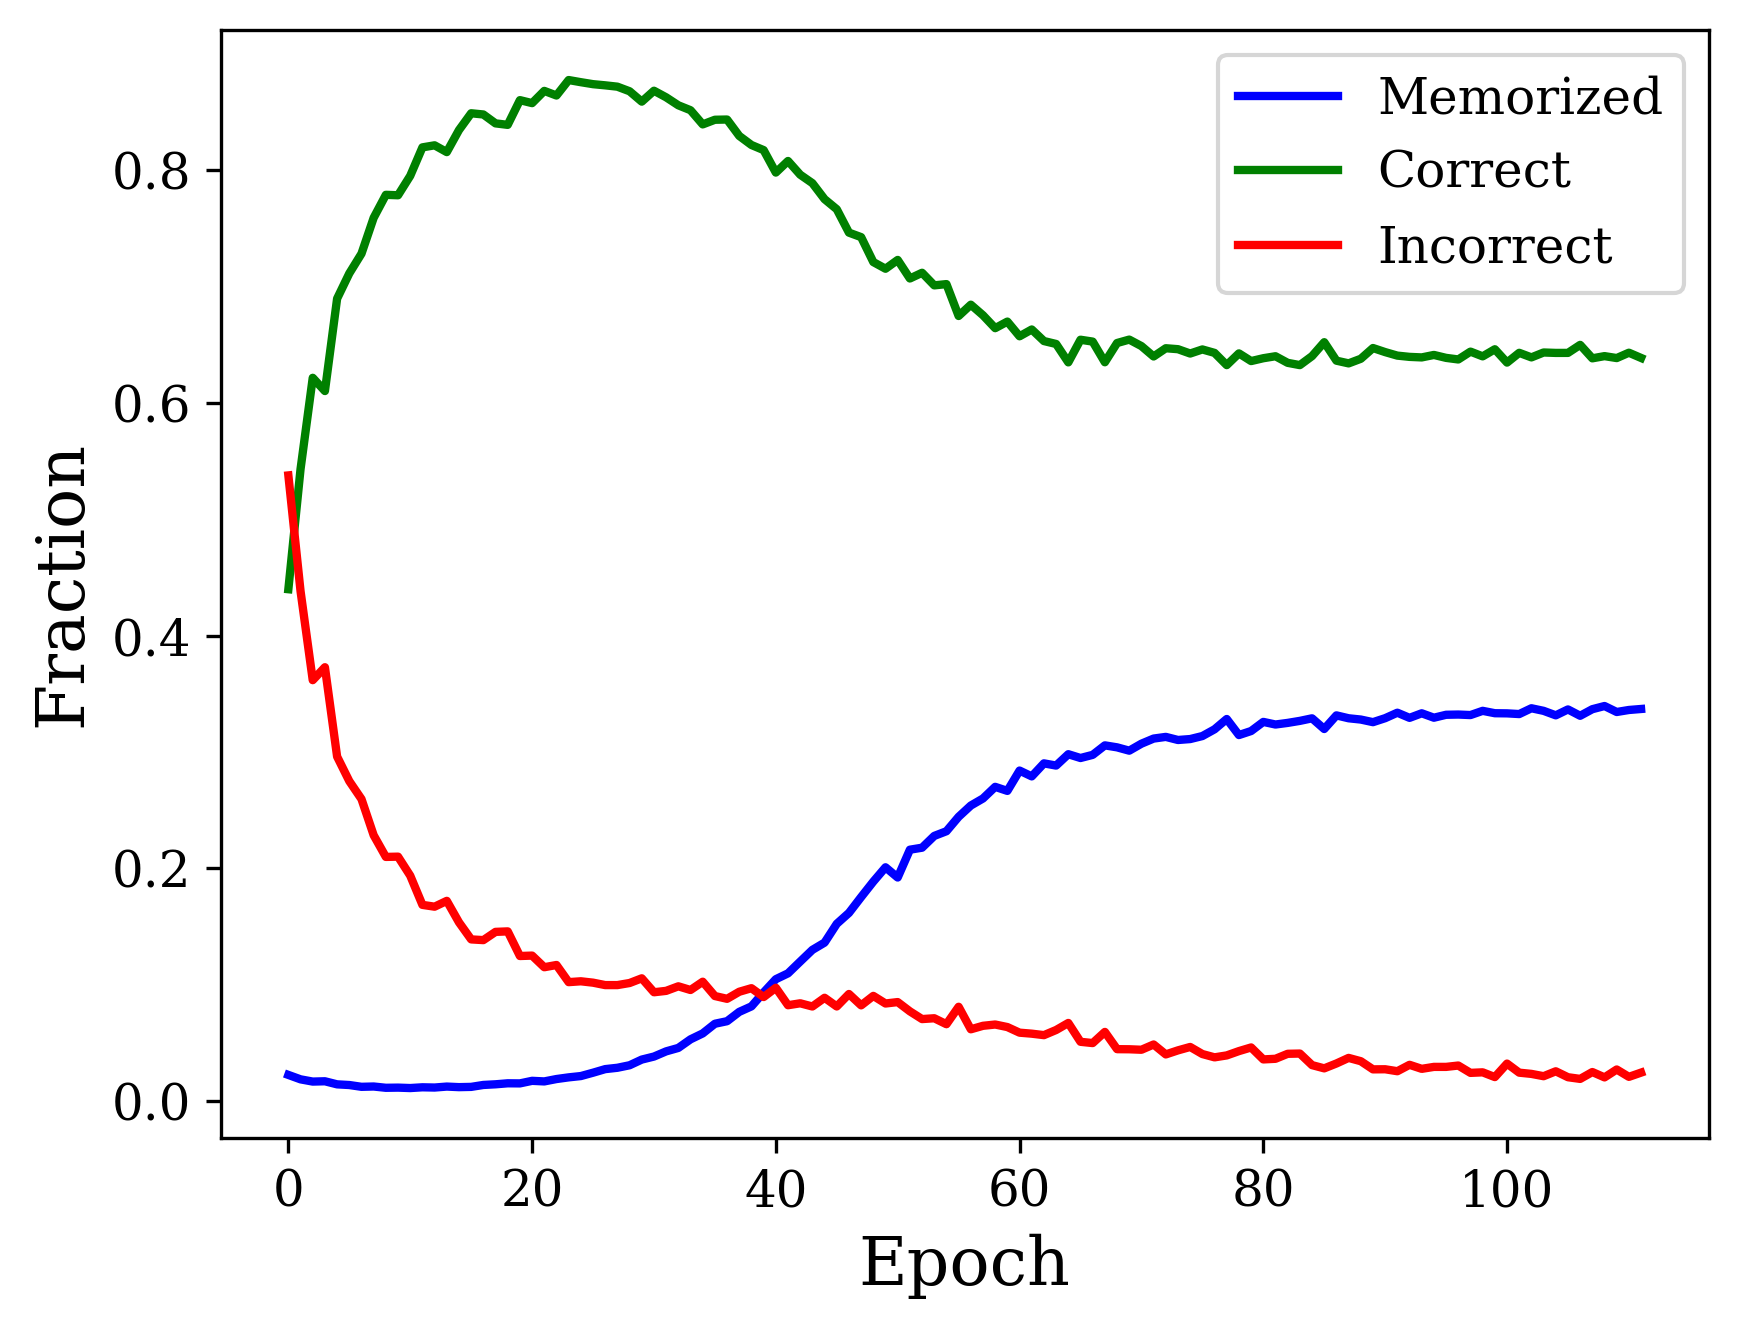
\includegraphics[width=\textwidth]{figures/memorized_correct_incorrect_04.png}
    \caption{symmetric noise, $\eta=0.4$}
    \label{fig:sub2}
  \end{subfigure}
  \caption{Training the ResNet-18 model on CIFAR10 with noisy labels results in memorization. Predicted labels are classified as \textit{correct} (predicted label matches the ground truth), \textit{memorized} (predicted label matches the incorrect noisy label), or \textit{incorrect} (predicted label matches neither the ground truth nor the noisy label).}
  \label{fig:memorization}
\end{figure}



\subsection{Noise Models}
To assess the algorithm, we generate synthetic noise.
The common noise types in the literature include:
\begin{itemize}
    \item \textbf{Class-Conditional Noise}: Label corruption depends only on the true class, often modeled by a noise transition matrix.
    \item \textbf{Instance-Dependent Noise}: Label corruption depends on both the true class and the input features $x_i$ \citep{prog_noise_iclr2021}
\end{itemize}


In this paper, we only work with class-conditional noise, as it is much simpler to simulate. Following standard practice, we divide noise into symmetric (uniform) and asymmetric (non-uniform) types:

\begin{itemize}
    \item \textbf{Symmetric noise:} For each training example, the true label is replaced with a label chosen randomly from the set of all labels (including the true one) with probability~$\eta$.
    \item \textbf{Asymmetric noise:} For each training example, the true label is replaced with a predetermined incorrect label (depending on the true class $y_i$) with probability~$\eta$. Typically, the incorrect label is chosen to be a similar or easily confusable class.
\end{itemize}

Asymmetric noise better models real-world label corruption, as annotators are more likely to confuse similar classes.

\subsection{ALSO}

\citet{also} proposed the following reformulation of Equation~\ref{eq:empirical}:
\begin{equation}
    \max_{\pi \in \Delta_{N-1}} \min_{\theta \in \Theta}
    \left\{
        \sum_{i=1}^{N}\pi_i f_i(\theta)
        + \frac{\tau}{2}\|\theta\|_2^2
        - \tau\text{KL}[\pi\|\hat{\pi}]
    \right\},
    \label{eq:also}
\end{equation}
where \(\tau > 0\) is the regularization parameter (temperature), \(\text{KL}[\cdot\|\cdot]\) denotes the KL-divergence between two distributions, and \(\hat{\pi}\) is a prior distribution of weights from \(\Delta_{N-1}\). A common choice for \(\hat{\pi}\) is the uniform distribution, \(\hat{\pi} = \mathcal{U}(\mathbf{1}, N)\). This formulation encourages higher weights for samples that are more difficult to classify correctly, helping to identify potentially mislabeled data. The authors solve the optimization problem in Equation~\ref{eq:also} using different variations of the Mirror-Prox algorithm, constructing the ALSO optimizer.


\section{Method}

\subsection{ALSO tweak}

We apply the ALSO optimizer to datasets with synthetic noise. However, we notice that assigning higher weights to mislabeled objects encourages the model to learn from them faster, leading to quicker overfitting. To counter this, we use a modified version of Equation~\ref{eq:also} in which the maximum over $\pi$ is replaced with a minimum. We observe that such a modification ensures that the model is much less prone to overfitting.

\subsection{Loss Modelling}

Following \citet{UnsupervisedLabelNoise}, we model the weights as a Beta mixture model, where the probability density function of the loss is given by $p(l) = \sum_{k=1}^2 w_k \cdot p(l|k)$. The two components correspond to weights for clean and corrupted objects. Here, $p(l|k)$ is the probability density function of a Beta distribution with parameters $\alpha_k$ and $\beta_k$. We fit a Beta Mixture Model to the ALSO weights using the same EM algorithm described in \citet{UnsupervisedLabelNoise}. We observe that the ALSO weights fit the Beta Mixture Model much better than the loss values from classical optimizers (see Figure~\ref{fig:loss_model}).

\begin{figure}[htbp]
  \centering
  \begin{subfigure}[b]{0.45\textwidth}
    \centering
    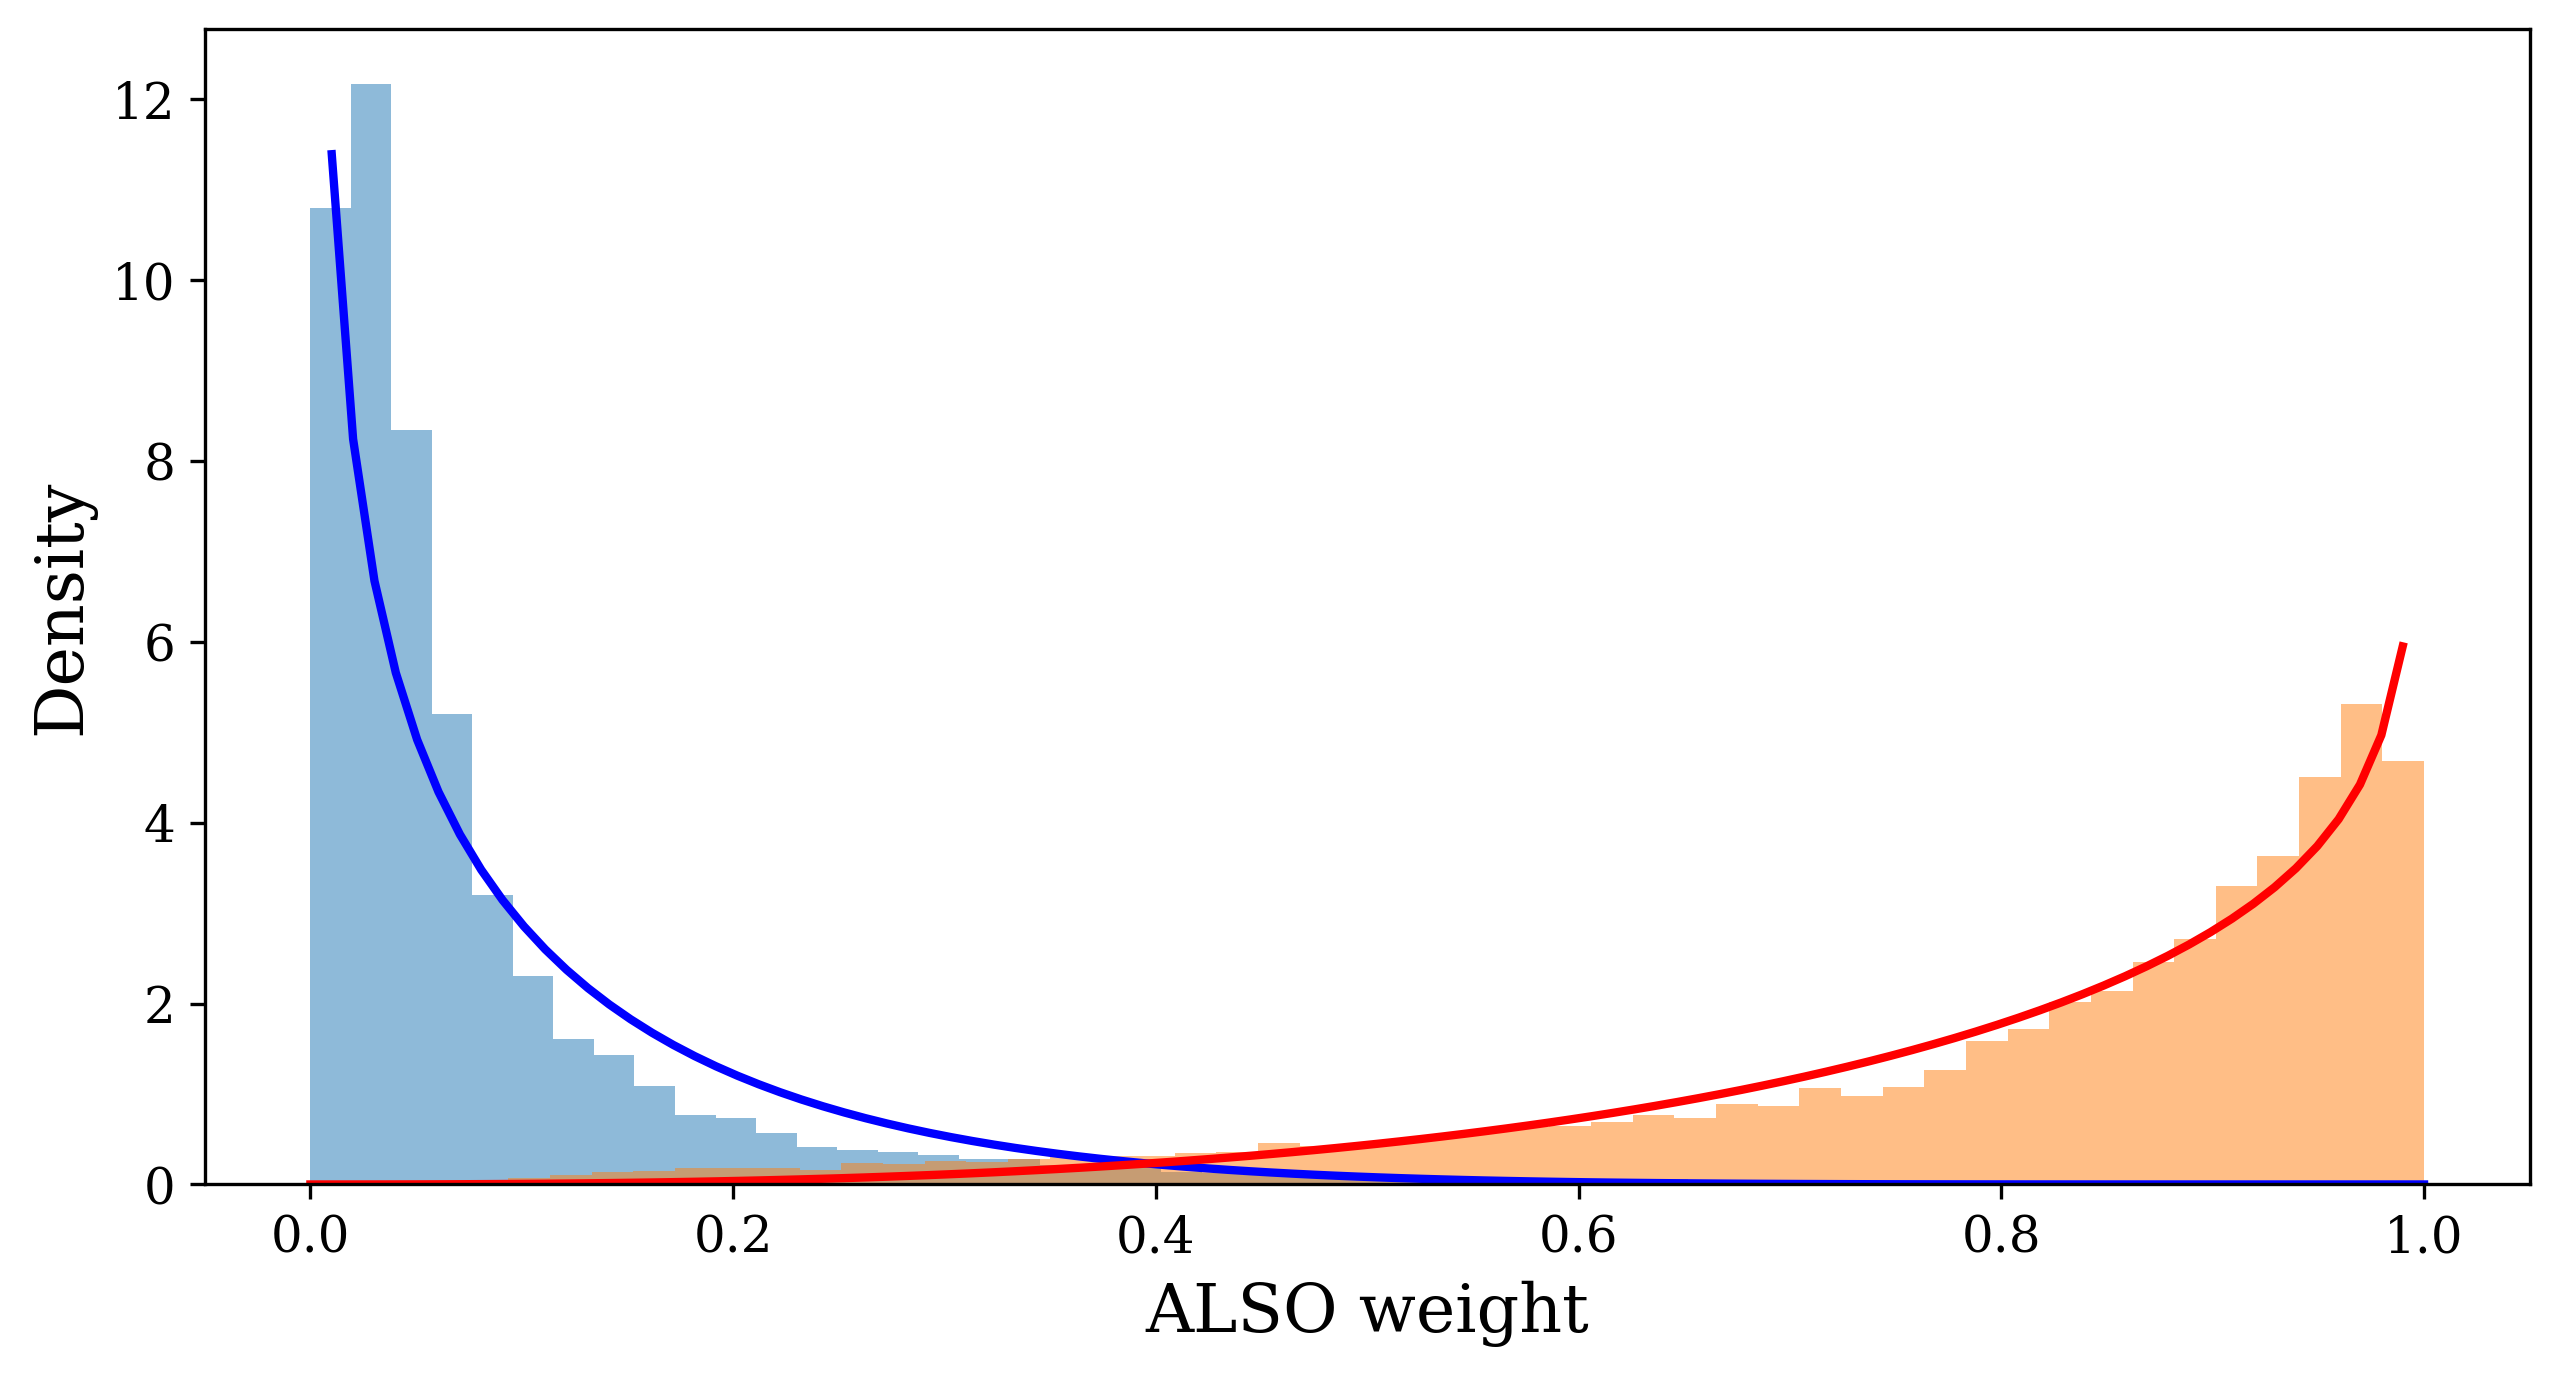
\includegraphics[width=\textwidth]{figures/minmin_weights.png}
    \caption{ALSO weights at the end of training}
    \label{fig:sub1}
  \end{subfigure}
  \hfill
  \begin{subfigure}[b]{0.45\textwidth}
    \centering
    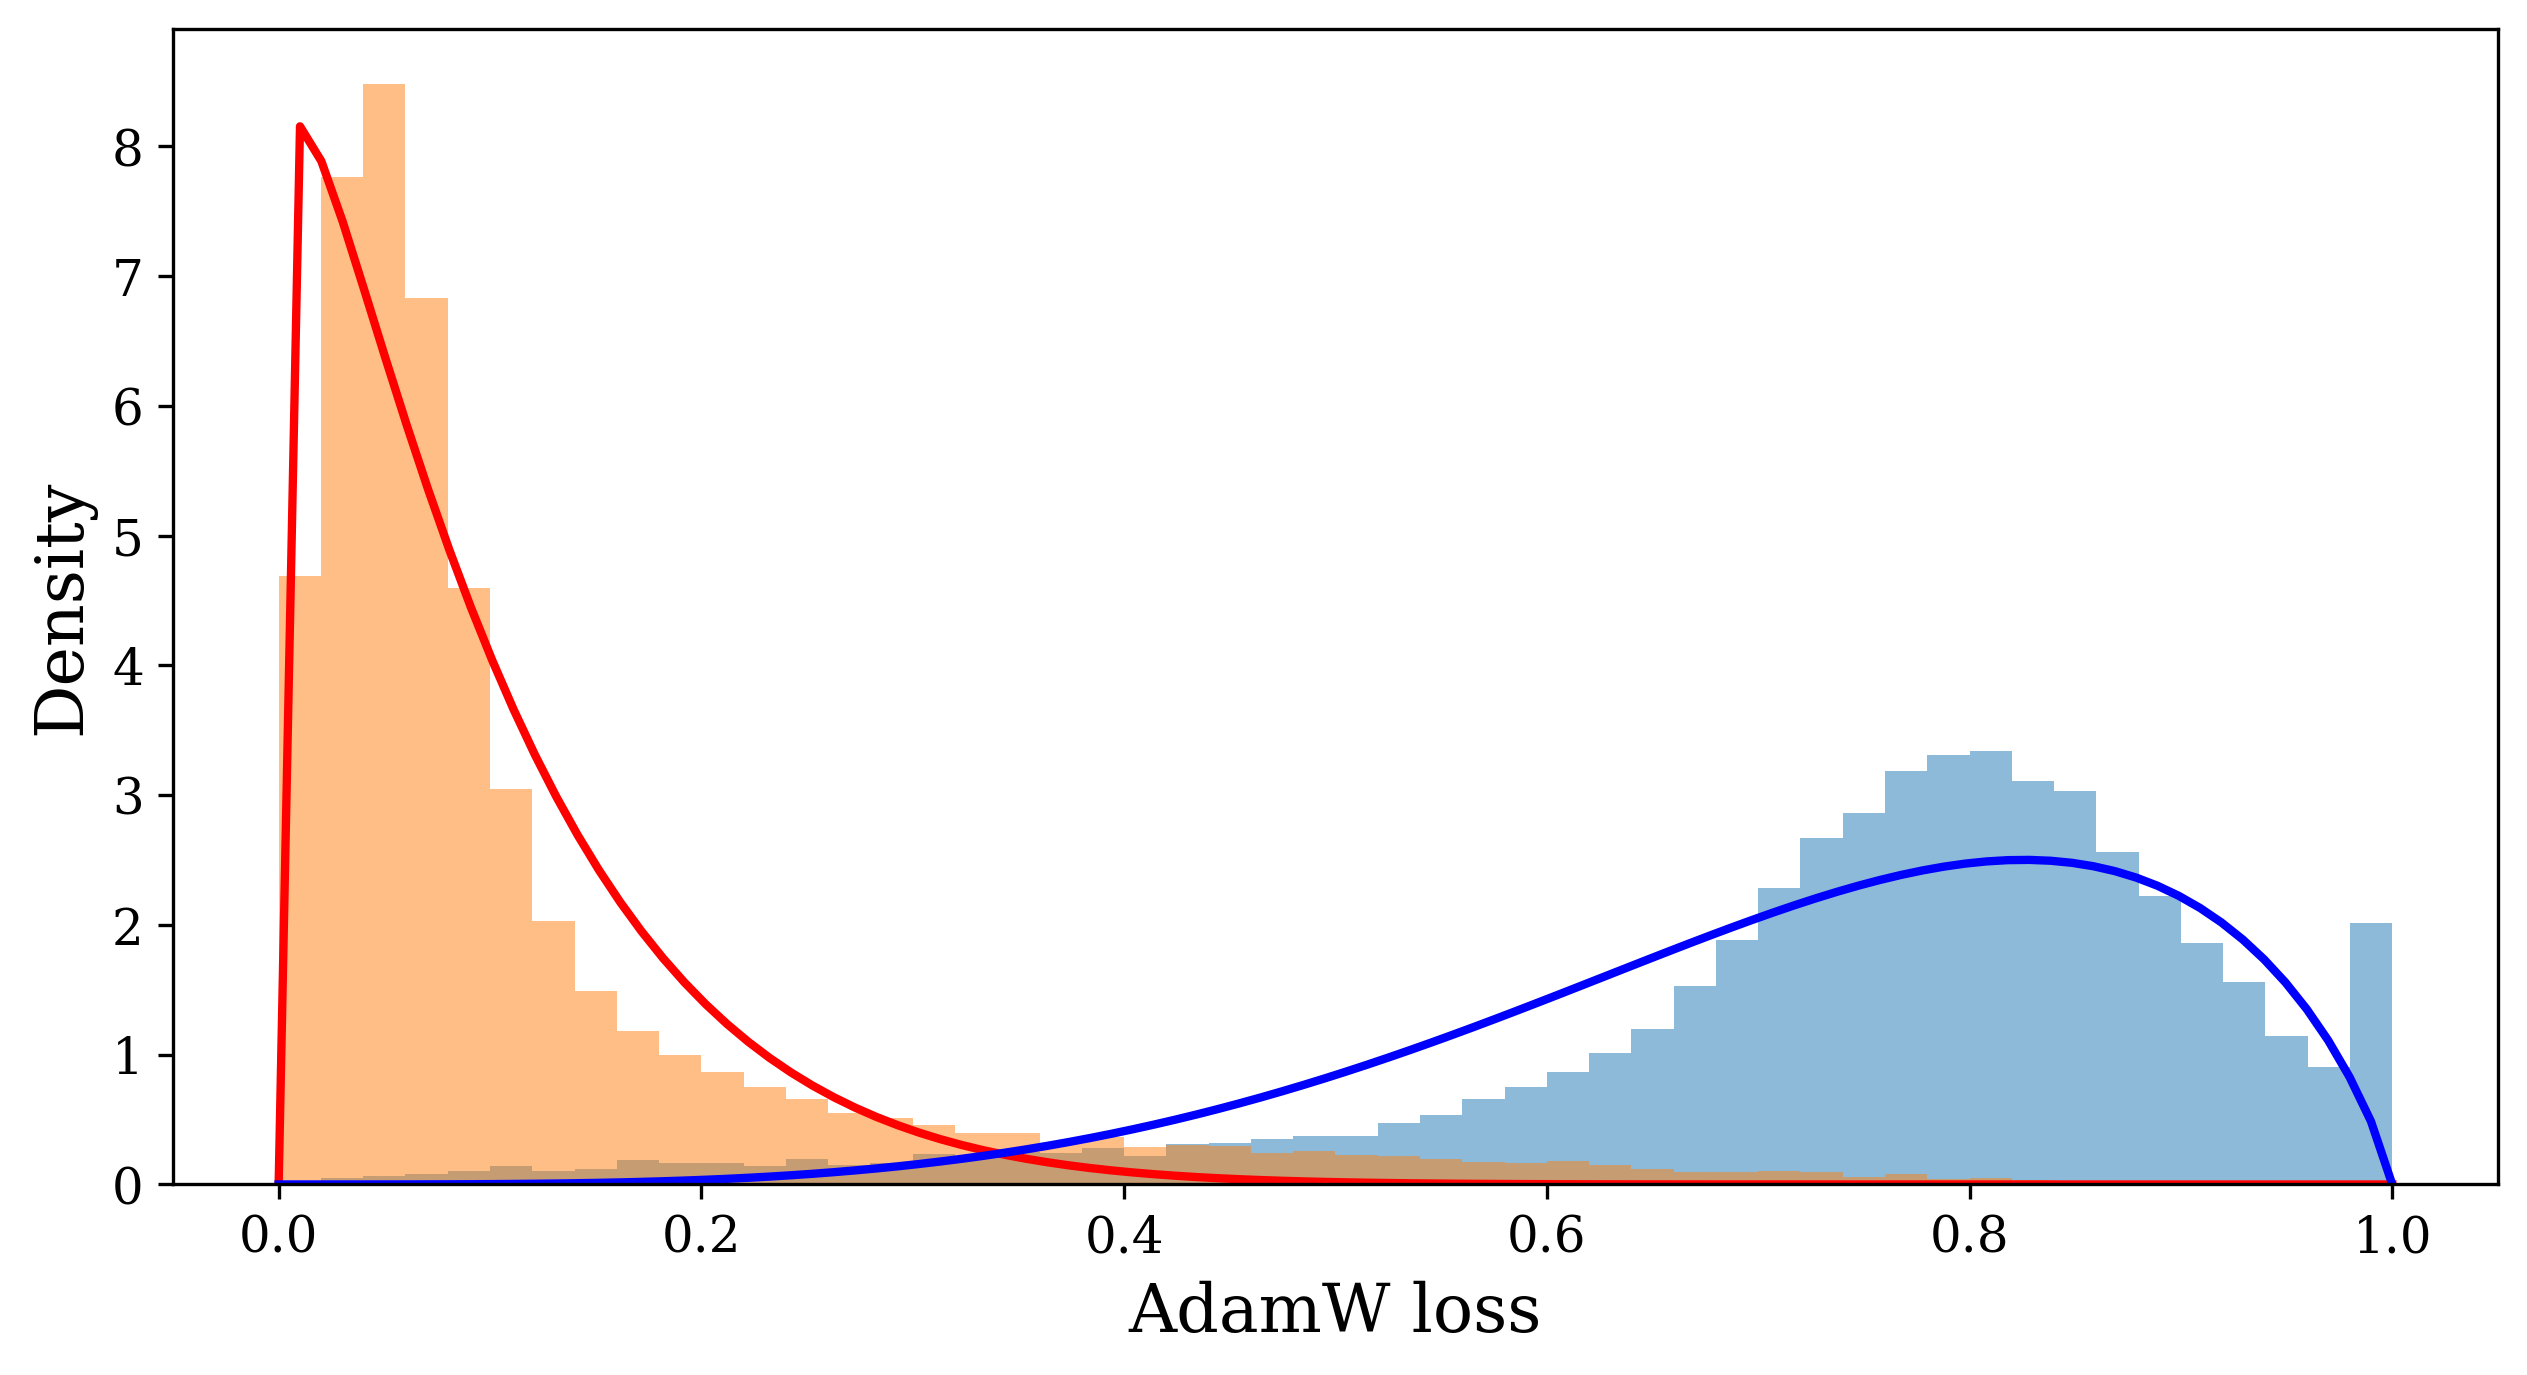
\includegraphics[width=\textwidth]{figures/adamw_losses.png}
    \caption{AdamW losses at "turning point"}
    \label{fig:sub2}
  \end{subfigure}
  \caption{Beta Mixture Model fitted to ALSO weights and AdamW losses under 0.4 symmetric noise. ALSO separates the classes better}
  \label{fig:loss_model}
\end{figure}

\section{Experiments}

\subsection{Setup}

We use the CIFAR10 dataset \citep{cifar} with standard augmentations (RandomCrop and RandomHorizontalFlip). For the network architecture we use ResNet-18 and ResNet-34 \citep{He_2016_CVPR} We add random symmetric or asymmetric noise at different levels. We train both AdamW and ALSO for 100 epochs and collect the training loss (in the case of AdamW) and the weights (in the case of ALSO) after each epoch. Then, we fit a Beta Mixture Model for each epoch and use it to estimate each object's probability of being corrupted.

We evaluate the performance of our approach using ROC-AUC, which measures how well our method separates clean and noisy labels after each epoch.

\subsection{Results}

\begin{figure}[H]
    \centering
    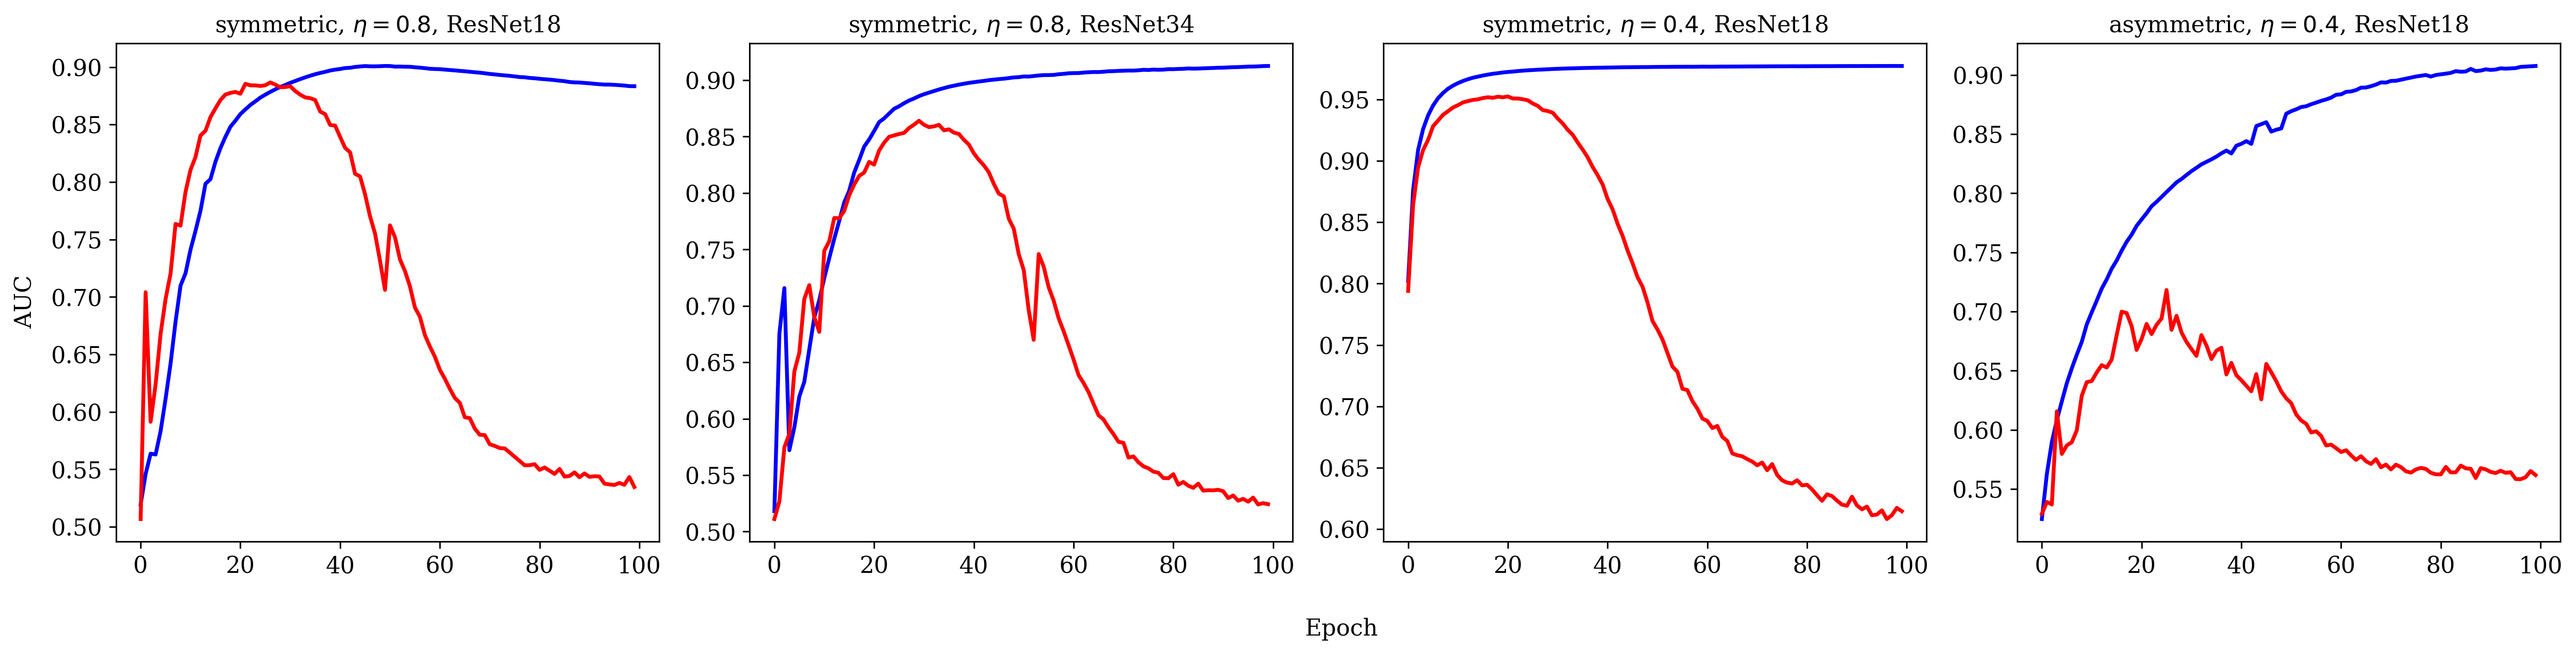
\includegraphics[width=1.0\linewidth]{figures/adam_vs_also.png}
    \caption{Measured ROC-AUC for different scenarios. The blue line represents ALSO, and the red line represents AdamW.}
    \label{fig:auc}
\end{figure}

As shown in Figure~\ref{fig:auc}, our method consistently outperforms the baseline approach in identifying mislabeled examples, achieving an AUC greater than 0.9 in all scenarios. An additional advantage of our method is its resistance to overfitting - as a result, the AUC remains stable and does not experience a sudden drop. This property is particularly valuable in practice, as it eliminates the need for early stopping that can be difficult to apply when a clean validation set is not available.

\section{Conclusion}

In this paper, we introduced an approach for identifying mislabeled examples in training data by leveraging a modified Adaptive Loss Scaling (ALSO) optimizer. We demonstrated that by changing the optimization objective of ALSO to minimize over sample weights, we can prevent the model from overfitting to noisy labels. By fitting a Beta Mixture Model to the learned sample weights, our method achieves superior separation between clean and noisy examples compared to approaches relying on loss values from standard optimizers like AdamW.

\bibliography{references}

\end{document}